\chapter{Zespołowe przedsięwzięcie inżynierskie}


Zespołowe przedsięwzięcie inżynierskie oznaczać będzie projekt, działanie podjęte w realizacji postawionego celu, realizowane zespołowo.\\\\
Projekt jest odpowiedzią na problem/potrzebę, w określonej przestrzeni życia.


\section{Członkowie zespołu z określeniem funkcji}
\begin{enumerate}
\item Piotr Jabloński - programista Java
\item Mirosława Pelc - programista Java
\item Mariusz Lorek - kierownik zespołu, testy programu, przygotowanie dokumentacji projektu
\end{enumerate}

\section{Uzasadnienie potrzeby realizacji projektu}
Celem zespołowego przedsięwzięcia jest przygotowanie programu który wspomoże zorganizowanie turnieju szachowego w którym wziąść może udział dowolna, nieznana wcześniej liczba zawodników. Czas trwania turnieju jest ograniczony przez organizatora. Turniej szachowy jest organizowany cyklicznie, dlatego stworzenie programu wspomagającego jego obsługę znacznie ułatwi przeprowadzanie kolejnych edycji.


\section{Cele projektu}

\begin{enumerate}
\item Napisanie programu umożliwiającego przeprowadzenie turnieju szachowego.
\item Przygotowanie instrukcji obsługi do programu dla użytkownika
\item Przygotowanie dokumentacji dla projektu
\end{enumerate}
 


\section{Zakres projektu}
\begin{enumerate}
	\item Stworzenie programu do wspomagania organiacji turnieju szachowego według wytycznych zleceniodawcy
	\item Stworzenie dokumentacji opisującej postępy prac nad tworzonym projektem z podziałem na czynności które ma wykonywać każdy z członków zespołu
\end{enumerate}
Program ma pozwalać na:
\begin{enumerate}
	\item Przeprowadzenie turnieju szachowego w systemie kołowym (każdy z każdym) - dwie rundy:
	\begin{itemize}
		\item eliminacje
		\item finał
	\end{itemize}
	\item Zapis stanu turnieju w dowolnym monencie
	
	\item Wprowadzenie do programu danych o uczestnikach
	\begin{itemize}
		\item imię
		\item nazwisko
		\item wiek
		\item kategoria szachowa
	\end{itemize}
	\item Edycja danych uczestnika
	\item Usunięcie uczestnika z listy uczestników turnieju 
	\item Podział uczestników turnieju na grupy zgodnie z wybranym kryterium, rosnąco lub malejąco:
	\begin{itemize}
		\item alfabetycznie
		\item według wieku
		\item ręcznie
		\item losowo
	\end{itemize}
	\item Ustalenie optymalnej liczby grup dla danej liczby uczestników turnieju
	\item Określenie ilości szachownic na których będzie rozgrywany turniej
	\item Określenie czasu trwania pojedyńczej rozgrywki
	
	\item Ustalanie uczestników każdego meczu - kolor pionków (biały, czarny) przydzielany do zawodników przed każdym spotkaniem 
	\item Punktowanie rozegranych spotkań
	\item Możliwość wyboru uczestników do rundy finałowej
\end{enumerate}


\section{Grupy docelowe}
Program przeznaczony dla organizatorów turniejów szachowych lub gier o zbliżonych zasadach (np. warcaby)  


\section{Struktura podziału prac (zadań) - WBS}
\begin{enumerate}
\item Zebranie informacji na temat sposobu przprowadzania turnieju szachowego od zleceniodawcy.
\begin{enumerate}
	\item Wybranie systemu w którym będzie przeprowadzany turniej.
	\item Przygotowanie regulaminu turnieju.
\end{enumerate}
\item Projekt programu.
\begin{enumerate}
\item Określenie jakie elementy muszą się znaleść w programie
\item Szablon programu
\item Wybór środowiska programistycznego
\item Rozdzielenie zadań dla programistów
\end{enumerate}
\item Tworzenie programu/aplikacji
\begin{enumerate}
\item Opracowanie narzędzi bazodanowych przechowujących informacje dotyczące turniejów
\item Przygotowanie elementów środowiska graficznego
\item Integracja narzędzi bazodanowych z elementami środowiska graficznego
\item Wstępna wersja programu
\item Testowanie
\begin{itemize}
\item testy uczestników projektu
\item testy zamawiającego program
\end{itemize}

\end{enumerate}
\item Eliminacja znalezionych błędów
\item Dodawanie kolejnych funkcji do programu
\item Końcowa wersja programu

\end{enumerate}

\section{Regulamin turnieju}
\begin{enumerate}
\item Obowiązują przepisy gry międzynarodowej federacji szachowej (fide).
\item Każdy z zawodników powinien się kierować zasadami fair play.
\item Zasady rozgrywki:
\begin{enumerate}
\item Turniej rozgrywany jest w dwóch fazach: grupowej i finałowej.\\
\item Tworzona jest lista startowa według przyjętych przez prowadzącego turniej kryteriów, domyślnie:
\begin{itemize}
\item kategoria szachowa 
\item wiek
\item alfabetycznie
\end{itemize}
\item Ilość grup jest zależna od liczby uczestników i ustala ją prowadzący.
\item Lista startowa dzielona jest na liczbę części równą liczbie grup
\item Następnie zawodnicy z każdej części są losowo rozmieszczani w grupach
\item W fazie grupowej prowadzone są rozgrywki, wedug zasady "każdy z każdym" w danej grupie
\item W fazie finałowej zawodnicy wyłonieni z grup (liczbę osób wychodzących z grup ustala prowadzący) grają między sobą.
\item Jeżeli zawodnicy grali ze sobą w rundzie eliminacyjnej to w finale przyjmuje się wynik rozgrywki z eliminacji
\item Czas trwania turnieju jest ograniczony, podany przez organizatora
\begin{itemize}
\item 10 minut na przyjmowanie zgłoszeń(rejestrację),
\item 10 minut na losowanie spotkań,
\item Na każdą rozgrywaną partię przypada 10 minut. Każdy zawodnik ma 5 minut na wykonanie swoich posunięć.
\end{itemize}
\item Zawodnicy mają do dyspozycji zegar analogowy lub cyfrowy z 2 tarczami lub wyświetlaczami umożliwiający odmierzanie czasu rozgrywki dla każdego z zawodników osobno
\item Za zajecie ustalonych przez prowadzącego miejsc w turnieju zawodnicy otrzymują nagrody przewidziane przez organizatora.
\item Jeśli prowadzący ustali, uczestnicy będą mieli obowiązek zapisywać swoje ruchy na przeznaczonych do tego kartach.
\item Każdy stanowisko do gry ma swój numer identyfikacyjny, który obowiązuje przy rozgrywkach.
\item W sali, w której obywa się turniej szachowy zawodnicy jak i widzowie muszą zachować bezwzględną ciszę, aby nie przeszkadzać graczom w rozgrywce.
\item Jeśli jakiś uczestnik turnieju lub widz będzie podpowiadał innemu uczestnikowi, zawodnik otrzymuje od prowadzącego ostrzeżenie, w wypadku powtórzenia się sytuacji gracz któremu pomoc została ponownie udzielona może zostać zdyskwalifikowany z dalszych rozgrywek przez prowadzącego.
\item W turnieju obowiązuje punktacja
\begin{itemize}
	\item Zwycięstwo - 1pkt
	\item Remis - 0,5pkt
	\item Porażka - 0pkt
	\item Punkty pomocnicze, wykorzystywane gdy kilku zawodników ma taką samą liczbę punktów głównych, przyznawane po zakończeniu etapu (eliminacji lub finału) według schematu:
	\begin{itemize}
		\item Punkty zawodników z którym dany zawodnik wygrał
		\item Remis - połowę punktów zawodników z którym dany zawodnik zremisował
		\item Porażka - Nie są przyznawane punkty pomocnicze
	\end{itemize}
	\end{itemize}
\end{enumerate}
\item W razie rezygnacji lub dyskwalifikacji zawodnika z turnieju, rozgrywki, które rozegrał nie zostają anulowane, a osoby, które się z nim spotykają w kolejnych rozgrywkach wygrywają walkowerem (otrzymują 1pkt za zwycięstwo)
\item W Sali zostało wydzielone pięć części:
\begin{enumerate}
\item Pierwsza, w której znajdują się tylko i wyłącznie osoby rozgrywające mecz
\item Druga, w której znajdują się widzowie bądź gracze, którzy obecnie nie rozgrywają żadnego spotkania
\item Trzecia, w której znajdują się stanowiska do gry w szachy poza turniejem
\item Czwarta, w której znajdują się gracze oczekujący na mecz
\item Piąta, w której znajduje się tylko i wyłącznie prowadzący turniej szachowy bądź osoby, które za zezwoleniem mogą znajdować się w tej strefie
\end{enumerate}
\item Zawodnicy, którzy nie grają lub czekają na swoją kolej w obrębie sali lub w niedalekiej odległości od niej w wypadku wezwania do rozgrywki powinni w trybie natychmiastowym zgłosić się do udziału w spotkaniu. W wypadku niestawienia się do rozegrania meczu zawodnik zostaję zdyskwalifikowany.
\item W przypadku, gdy:
\begin{itemize}
\item Zawodnik utrudnia przeprowadzanie rozgrywek może zostać zdyskwalifikowany z turnieju lub wyproszony z sali przez Prowadzącego.
\item Widz utrudnia przeprowadzanie rozgrywek może zostać wyproszony z sali przez Prowadzącego.
\end{itemize}
\item Udział w turnieju szachowym jest równoznaczny z zaakceptowaniem regulaminu
\end{enumerate}
\section{Rozgrywki w systemie szwajcarskim - zrezygnowano w czasie trwania projektu}

\textbf{System szwajcarski} - W systemie szwajcarskim z góry określa się liczbę rund, które należy rozegrać.\\
Na rundę składają się bezpośrednie pojedynki (gry) rozgrywane jednocześnie.\\ Za zwycięstwo w grze uczestnik otrzymuje jeden punkt, za remis pół punktu (punktacja może być inna).\\
Dobór par przeciwników w kolejnych rundach zależy od wyników uzyskanych w poprzednich. Pary dobiera się w miarę możliwości spośród tych uczestników, którzy dotychczas zdobyli jednakową liczbę punktów.\\
Jeśli liczba uczestników zawodów jest nieparzysta, w każdej rundzie jeden z uczestników z najmniejszym dorobkiem punktowym, który jeszcze nie pauzował, otrzymuje wolny los (tzw. bye) czyli dostaje punkt bez gry.\\
Kojarzenie par w kolejnych rundach jest dość skomplikowane, ponieważ system musi wykluczyć możliwość dwukrotnego spotkania się tych samych przeciwników.\\
Dodatkową komplikacją jest konieczność zapewnienia "sprawiedliwego" przydziału kolorów bierek w kolejnych pojedynkach.

\subsection{Wytyczne Międzynarodowej Federacji Szachowej (FIDE)}
Międzynarodowa Federacja Szachowa (FIDE) opracowała precyzyjny regulamin rozgrywania zawodów systemem szwajcarskim. Przed zawodami zawodnicy są uszeregowani w kolejności punktacji rankingowej odzwierciedlającej aktualną siłę gry każdego zawodnika. Listy rankingowe są publikowane co miesiąc. Przed kojarzeniem I rundy listę tę dzieli się na dwie części. W górnej połowie listy znajdują się zawodnicy najwyżej zaszeregowani, w dolnej – pozostali. W pierwszej rundzie zawodnik z nr 1 spotka się z zawodnikiem najwyżej zaszeregowanym w dolnej grupie i następnie kolejni według tej zasady. Kolor bierek dla pierwszej pary jest losowany, następne pary zawodników otrzymają kolory bierek odmienne.\\\\
\textbf{Podstawowe zasady kojarzenia par w systemie szwajcarskim zostały w regulaminie określone w następujący sposób:}
\begin{enumerate}
\item dwóch zawodników nie może się spotkać więcej niż jeden raz;
\item zawodnik, który otrzymał punkt bez gry nie może otrzymać wolnego losu;
\item zawodnik może rozegrać jednym kolorem dwie partie z rzędu (lub trzy jeżeli trzecia to ostatnia partia turnieju);
\item kojarzenie do następnej rundy odbywa się w ramach grup punktowych z tą samą liczbą punktów, a jeśli to dla niektórych zawodników jest niemożliwe różnica punktowa pomiędzy kojarzonymi zawodnikami musi być najmniejsza z możliwych;
\item tak wielu zawodnikom, jak to tylko możliwe, należy przydzielić oczekiwany kolor; jest to kolor, którym rozegrali mniej partii niż drugim kolorem, a w przypadku równej liczby partii jest to kolor odmienny od koloru poprzedniej rundy (jeśli dwóch skojarzonych zawodników oczekuje na ten sam kolor – musi być spełniony warunek pkt 3, a oczekiwany kolor bierek otrzyma zawodnik, który ma bardziej nierówny przydział kolorów z poprzednich rund, dodatkowo – jeśli dwóch skojarzonych zawodników ma identyczną historię przydziału koloru z poprzednich rund – oczekiwany kolor otrzyma zawodnik wyżej zaszeregowany na liście);
\item zawodnik, który grał w poprzedniej rundzie z zawodnikiem o większej (mniejszej) liczbie punktów nie powinien być ponownie skojarzony z zawodnikiem o większej (mniejszej) liczbie punktów;
\item zawodnik, który grał dwie rundy wcześniej z zawodnikiem o większej (mniejszej) liczbie punktów nie powinien być ponownie skojarzony z zawodnikiem o większej (mniejszej) liczbie punktów.
\end{enumerate}
Zasady 1-2 \textbf{są bezwarunkowe}, tzn. kojarzenie musi spełnić każdy z tych warunków. Zasady 3-4 są również \textbf{bezwarunkowe z wyjątkiem ostatniej rundy}, kiedy wolno je złamać, jeśli dzięki temu uda się skojarzyć więcej par, w których zawodnicy będą mieli taką samą liczbę punktów. Zasady 5-8 są uszeregowane według ważności i muszą być stosowane we wszystkich przypadkach, w których nie są sprzeczne z zasadami ważniejszymi. Regulamin FIDE zawiera szczegółowy opis algorytmu kojarzenia par.

\subsection{Zalety systemu szwajcarskiego}
Ogromną zaletą systemu szwajcarskiego jest \textbf{możliwość rozegrania turnieju w jednej grupie z udziałem dużej liczby zawodników}. W turniejach szachowych rozgrywanych tym systemem nierzadko bierze udział \textbf{kilkuset zawodników o różnym poziomie gry}. Początkujący mogą w bezpośrednim pojedynku spotkać się z arcymistrzami, w jednym turnieju mają szansę pokonać zawodników uznawanych za silniejszych i szybko awansować w szachowej hierarchii. Ważne jest również, że \textbf{jedna słabsza gra nie przekreśla szans zawodnika}. Takich możliwości nie daje ani system kołowy (ze względu na dużą liczbę koniecznych gier) ani pucharowy, który eliminuje zawodnika po pierwszej porażce.

\subsection{Wady systemu szwajcarskiego}
Wadą systemu szwajcarskiego jest \textbf{spory wpływ czynnika losowego}, którego znaczenie ogranicza się poprzez ustalenie początkowej kolejności zawodników według siły gry (zazwyczaj na podstawie rankingu). System szwajcarski jest również \textbf{znacznie mniej obiektywny od systemu kołowego.} Zawodnik, który przegrywając w pierwszych rundach, w końcowych zdobywał punkty na słabszych przeciwnikach może w ostatecznej klasyfikacji wyprzedzić zawodnika, który dobrze grał z silniejszymi, lecz w końcowych rundach zdobył mało punktów. \textbf{Decydujące znaczenie ostatniej rundy stanowi o specyficznej atrakcyjności systemu szwajcarskiego.}
System ten nie sprawdza się też dobrze, w momencie \textbf{gdy liczba zawodników jest niewiele większa od liczby rund do rozegrania.} Wówczas w końcowych rundach spotkać się mogą zawodnicy, których różnica punktów jest spora.

%Diagram sieciowy ukazuje zależności czasowe, węzły (aktywności), krawędzie (zależności czasowe).


\section{Harmonogram}
\subsection{Harmonogram prac poszczególnych członków zespołu}
\textbf{Mirosława Pelc oraz Piotr Jabłoński wspólna praca programistyczna\\
Mirosława Pelc - Odpowiedzialna w głównej mierze za interfejs graficzny\\
Piotr Jabłoński - Programowanie, algorytmy\\}
\begin{tabular}{|p{9cm}|l|p{3cm}|} \hline
Zadanie & Data rozpoczecia & Data zakończenia\\ \hline
Przygotowanie klas odpowiadających za uczestnika, turniej, rozgrywkęzygotowanie klas odpowiadających za uczestnika, turniej, rozgrywkę & 6.10.2015 & 20.10.2015 \\ \hline
Wyszukikawanie możliwych do wykorzystania elementów dostępnych w bibliotekach graficznych dla języka JAVA& 6.10.2015 & 20.10.2015 - zadanie ciągłe wykonywane przez cały czas trwania projektu\\ \hline
Integracja z bazą danych SQLite do przechowywania uczestników& &\\
Integracja z bazą danych SQLite do przechowywania turniejów&20.10.2015&27.10.2015\\
Integracja z bazą danych SQLite do przechowywania wyników pojedynczych rozgrywek&&\\ \hline
tabela - lista uczestników&27.10.2015&3.11.2015\\ \hline
dodawanie nowego uczestnika&27.10.2015&3.11.2015\\ \hline
usuwanie uczestnika&3.11.2015&10.11.2015\\ \hline
edycja uczestnika&3.11.2015&10.11.2015\\ \hline
dodawanie losowego uczestnika&10.11.2015&17.11.2015\\ \hline
symulacja ilości rozgrywek dla danej liczby uczestników, typu turnieju (systemem szwajcarskim / eliminacje grup)&10.11.2015&17.11.2015\\ \hline
podział graczy na grupy wg listy sortowanej po ustalanych przez prowadzącego turniej (dynamicznie w programie) warunkach takich, jak: kategoria zawodnika, wiek, nazwisko, imię lub przydział manualny&17.11.2015&24.11.2015\\ \hline
tworzenie początkowej listy graczy (sortowanie) do turnieju rozgrywanego systemem szwajcarskim (sortowanie po kategorii, wieku, nazwisko, imię)&17.11.2015&24.11.2015\\ \hline
dobieranie zawodników w pary dla systemu kołowego z eliminacjami w grupach - eliminacje
wybór zawodników przechodzących do finałów w rozgrywkach z eliminacjami
dobieranie zawodników w pary dla systemu kołowego z eliminacjami w grupach - finały&24.11.2015&1.12.2015\\ \hline
dobór zawodników w systemie kołowym (4 tyg!)&&\\ \hline 
lista wyników dla turnieju rozgrywanego systemem kołowym z eliminacjami&1.12.2015&8.12.2015\\ \hline
lista wyników dla turnieju rozgrywanego systemem szwajcarskim&&\\ \hline 
zastosowanie programu do prowadzednia kilku turniejów jednocześnie&&\\ \hline
usprawnienia ergonomii interfejsu&&praca ciągła do końca trwania projektu\\ \hline
usprawnienia estetyczne interfejsu&&praca ciągła do końca trwania projektu\\ \hline

\end{tabular}

\begin{tabular}{|p{9cm}|l|p{3cm}|} \hline
Zadanie & Data rozpoczecia & Data zakończenia\\ \hline
Przygotowanie dokumentacji dla projektu&&cały czas trwania projektu\\ \hline
Rozmowa ze zleceniodawcą na temat projektu &&20.10.2015\\ \hline
Wybór systemu w którym przeprowadzany będzie turniej &&27.10.2015\\ \hline
Okreslenie regulaminu turnieju (czas trwania,  system rozgrywego, określenie zasad uczestnictwa w turnieju, powody do dyskwalifikacji) &&3.11.2015\\ \hline
Opis repozytorium GitHub wykorzystywanego do pracy w projekcie &&17.11.2015\\ \hline
Przygotowywanie kolejnych części dokumentacji na podstawie informacji dostarczonych przez pozostałych członków zespołu&&\\ \hline
Testowanie kolejnych wersji  programu, wyszukiwanie błędów sugestie na temat usprawnień - praca ciągła, do końca trwania projektu&&\\ \hline
Konsultację ze zleceniodawcą na temat ewentualnych poprawek, dodawania nowych funkcjonalności wymaganych przez zleceniodawcę.&&\\ \hline 
\end{tabular}

%\section{Dokumentacja}
Przygotowanie środowiska do równoległego opracowania dokumentacji projektu i realizacji przydzielonych zadań poszczególnym członkom zespołu projektowego.

%\subsection[Edycja plików dokumentacyjnych]{Edycja plików dokumentacyjnych - każdy członek zespoły niezależnie}
%Każdy z członków zespołu edytuje swój plik \LaTeX{} (czlonkowie/nrCzlonka/main.tex) i~umieszcza w nim całość analiz i wyników, które pozwoliły mu zrealizować przydzielone zadanie. Wszystkie pliki graficzne, każdy niezależnie umieszcza w swoim katalogu (czlonkowie/nrCzlonka).

%Pierwszą linia w pliku (czlonkowie/nrCzlonka/main.tex), zawiera imię i nazwisko opracowującego członka zespołu:
%\item Rodzaj zadania [Przygotowanie przestrzeni do zespołowej pracy]
%\item Data rozpoczęcia [2014-11-01]
%\item Data zakończenia [2014-11-02]
%\item Aktualny status [zaplanowane do realizacji, w trakcie realizacji, zakończone]
%\item dokładny opis realizowanego zadania [powinien zawierać opis, rysunki, tabele, kody napisanych programów]
%\end{itemize}

%Poniżej znajduje się przykładowy listing dla skróconych dwóch zadań:
%\begin{lstlisting}
%\zadanieprojektowe{Przygotowanie dokumentacji}{2014-11-01}{2014-11-02}{w trakcie do realizacji}

%Poniżej opisujemy całe zadanie zgodnie z konwencją poznaną na NI.
%Poniżej opisujemy całe zadanie zgodnie z konwencją poznaną na NI.

%Poniżej opisujemy całe zadanie zgodnie z konwencją poznaną na NI. 

%następne zadanie
%\zadanieprojektowe{Przygotowanie dokumentacji}{2014-11-03}{2014-11-03}{zakończone}
%\begin{figure}[H]
%\includegraphics[width=\textwidth]{czlonkowie/1/studzienkizDziura.jpg}
%\end{figure}
%\end{lstlisting}


\subsubsection{Obsługa GitHuba}
Repozytorium wykorzystywane w projekcie to "GitHub" aby zacząć korzystać z tego repozytorium należy najpierw założyć konto w serwisie \href{https://github.com}{https://github.com}
Wybieramy opcję "Sing up" i wypełnamy formularz rejestracyjny
\begin{figure}[H]
	\centering
	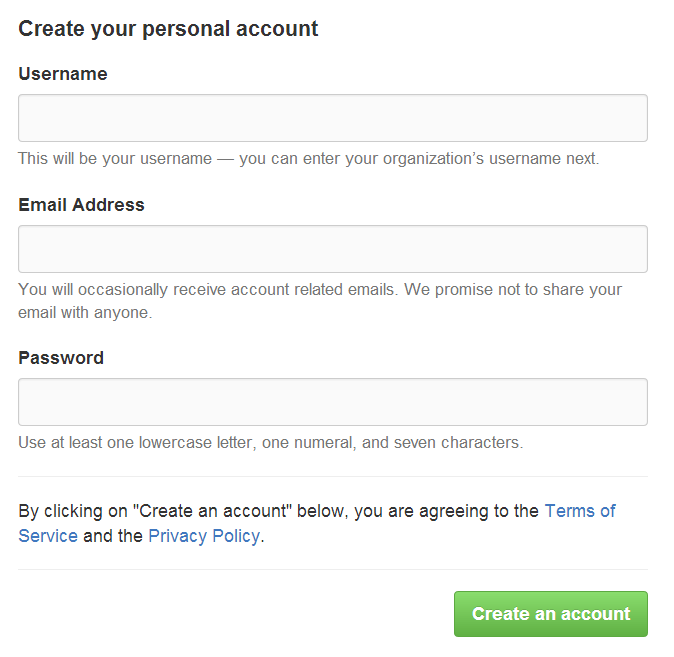
\includegraphics {fig/rejestracja}
	\caption{Formularz rejestracyjny repozytorium GitHub}
	\label{fig:rejestracja}
\end{figure}
Nastepnie z menu na górze po prawej stronie wybieramy opcję "New repository"
\begin{figure}[H]
	\centering
	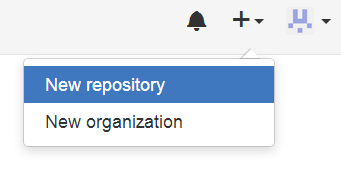
\includegraphics{fig/new_project}
	\caption{Tworzenie nowego repozytorium}
	\label{fig:new_project}
\end{figure}
Uzupełniamy dane dotyczące projektu. Musimy mu nadać nazwę, możemy opcjonalnie dodać opis tworzonego repozytorium, oraz zdecydować czy projekt będzie publiczny czy prywatny

\begin{figure}[H]
	\centering
	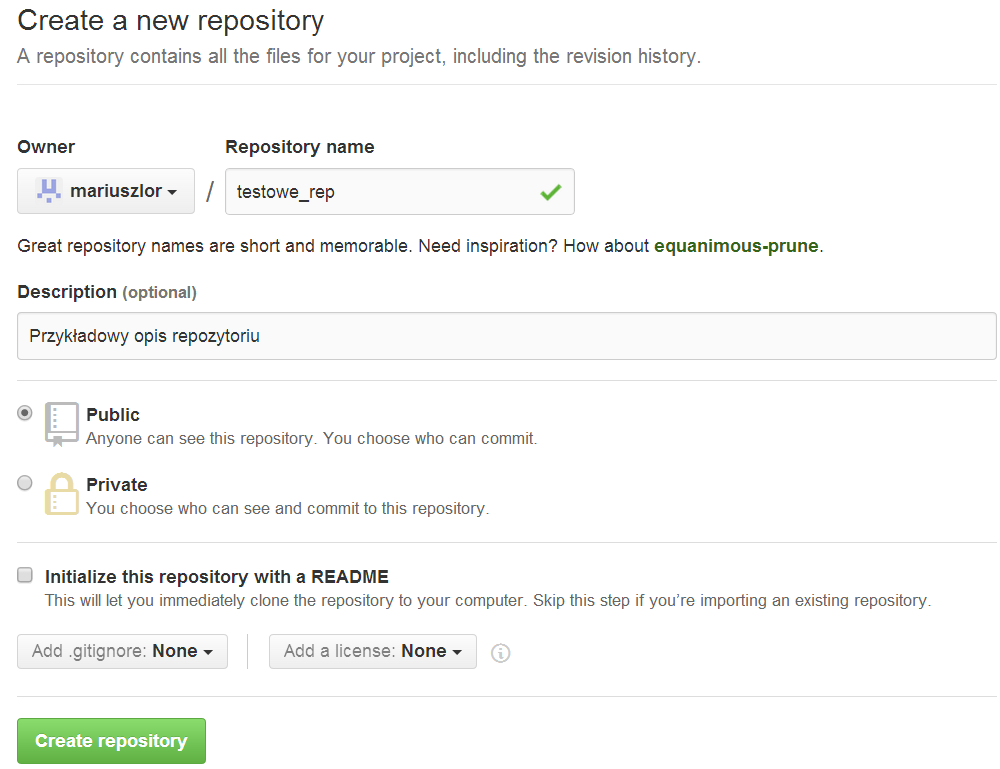
\includegraphics{fig/new_project_2}
	\caption{Uzupełniamy dane na temat projektu}
	\label{fig:new_project2}
\end{figure}
Teraz możemy dodać kolejnych uczestników projektu wybierając z menu opcję "New collaborator"
Uczestników możemy wyszukiwać  według róznych kryteriów
\begin{figure}[H]
	\centering
	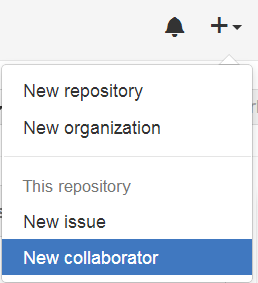
\includegraphics{fig/collaborator}
	\caption{Dodawanie nowego uczestnika projektu}
	\label{fig:collaborator}
\end{figure}
\begin{figure}[H]
	\centering
	
\includegraphics{fig/add_collaborator}
	\caption{Mamy możliwość wyszukiwania nowych członków według różnych kryteriów}
	\label{fig:add_collaborator}
\end{figure}
Aby mieć możliwość wysyłania plików do repozytorium musimy zainstalować program na swoim systemie w tym celu wchodzimy na stronę \href{https://desktop.github.com/}{https://desktop.github.com/}.\\ Program możemy zainstalować w systemach:
\begin{enumerate}
\item Windows 7
\item Windows 8/8.1
\item Windows 10
\end{enumerate}
Starsze wersję systemów operacyjnych nie są wspierane\\
Dostępna jest również wersja dla komputerów MAC z systemem OS X 10.9 lub nowszym
\begin{figure}[H]
	\centering
	
\includegraphics{fig/gitdownload}
	\caption{Przycisk umożliwiający pobranie programu}
	\label {fig:gitdownload} 
\end{figure}

